%  LaTeX support: latex@mdpi.com 
%  For support, please attach all files needed for compiling as well as the log file, and specify your operating system, LaTeX version, and LaTeX editor.

%=================================================================
\documentclass[algorithms,article,accept,moreauthors,pdftex]{Definitions/mdpi} 

% For posting an early version of this manuscript as a preprint, you may use "preprints" as the journal and change "submit" to "accept". The document class line would be, e.g., \documentclass[preprints,article,accept,moreauthors,pdftex]{mdpi}. This is especially recommended for submission to arXiv, where line numbers should be removed before posting. For preprints.org, the editorial staff will make this change immediately prior to posting.


%testestestest

%--------------------
% Class Options:
%--------------------
%----------
% journal
%----------
% Choose between the following MDPI journals:
% acoustics, actuators, addictions, admsci, adolescents, aerospace, agriculture, agriengineering, agronomy, ai, algorithms, allergies, analytica, animals, antibiotics, antibodies, antioxidants, appliedchem, applmech, applmicrobiol, applnano, applsci, arts, asi, atmosphere, atoms, audiolres, automation, axioms, batteries, bdcc, behavsci, beverages, biochem, bioengineering, biologics, biology, biomechanics, biomedicines, biomedinformatics, biomimetics, biomolecules, biophysica, biosensors, biotech, birds, bloods, brainsci, buildings, businesses, cancers, carbon, cardiogenetics, catalysts, cells, ceramics, challenges, chemengineering, chemistry, chemosensors, chemproc, children, civileng, cleantechnol, climate, clinpract, clockssleep, cmd, coatings, colloids, compounds, computation, computers, condensedmatter, conservation, constrmater, cosmetics, crops, cryptography, crystals, curroncol, cyber, dairy, data, dentistry, dermato, dermatopathology, designs, diabetology, diagnostics, digital, disabilities, diseases, diversity, dna, drones, dynamics, earth, ebj, ecologies, econometrics, economies, education, ejihpe, electricity, electrochem, electronicmat, electronics, encyclopedia, endocrines, energies, eng, engproc, entropy, environments, environsciproc, epidemiologia, epigenomes, fermentation, fibers, fire, fishes, fluids, foods, forecasting, forensicsci, forests, fractalfract, fuels, futureinternet, futuretransp, futurepharmacol, futurephys, galaxies, games, gases, gastroent, gastrointestdisord, gels, genealogy, genes, geographies, geohazards, geomatics, geosciences, geotechnics, geriatrics, hazardousmatters, healthcare, hearts, hemato, heritage, highthroughput, histories, horticulturae, humanities, hydrogen, hydrology, hygiene, idr, ijerph, ijfs, ijgi, ijms, ijns, ijtm, ijtpp, immuno, informatics, information, infrastructures, inorganics, insects, instruments, inventions, iot, j, jcdd, jcm, jcp, jcs, jdb, jfb, jfmk, jimaging, jintelligence, jlpea, jmmp, jmp, jmse, jne, jnt, jof, joitmc, jor, journalmedia, jox, jpm, jrfm, jsan, jtaer, jzbg, kidney, land, languages, laws, life, liquids, literature, livers, logistics, lubricants, machines, macromol, magnetism, magnetochemistry, make, marinedrugs, materials, materproc, mathematics, mca, measurements, medicina, medicines, medsci, membranes, metabolites, metals, metrology, micro, microarrays, microbiolres, micromachines, microorganisms, minerals, mining, modelling, molbank, molecules, mps, mti, nanoenergyadv, nanomanufacturing, nanomaterials, ncrna, network, neuroglia, neurolint, neurosci, nitrogen, notspecified, nri, nursrep, nutrients, obesities, oceans, ohbm, onco, oncopathology, optics, oral, organics, osteology, oxygen, parasites, parasitologia, particles, pathogens, pathophysiology, pediatrrep, pharmaceuticals, pharmaceutics, pharmacy, philosophies, photochem, photonics, physchem, physics, physiolsci, plants, plasma, pollutants, polymers, polysaccharides, proceedings, processes, prosthesis, proteomes, psych, psychiatryint, publications, quantumrep, quaternary, qubs, radiation, reactions, recycling, regeneration, religions, remotesensing, reports, reprodmed, resources, risks, robotics, safety, sci, scipharm, sensors, separations, sexes, signals, sinusitis, smartcities, sna, societies, socsci, soilsystems, solids, sports, standards, stats, stresses, surfaces, surgeries, suschem, sustainability, symmetry, systems, taxonomy, technologies, telecom, textiles, thermo, tourismhosp, toxics, toxins, transplantology, traumas, tropicalmed, universe, urbansci, uro, vaccines, vehicles, vetsci, vibration, viruses, vision, water, wevj, women, world 

%---------
% article
%---------
% The default type of manuscript is "article", but can be replaced by: 
% abstract, addendum, article, book, bookreview, briefreport, casereport, comment, commentary, communication, conferenceproceedings, correction, conferencereport, entry, expressionofconcern, extendedabstract, datadescriptor, editorial, essay, erratum, hypothesis, interestingimage, obituary, opinion, projectreport, reply, retraction, review, perspective, protocol, shortnote, studyprotocol, systematicreview, supfile, technicalnote, viewpoint, guidelines, registeredreport, tutorial
% supfile = supplementary materials

%----------
% submit
%----------
% The class option "submit" will be changed to "accept" by the Editorial Office when the paper is accepted. This will only make changes to the frontpage (e.g., the logo of the journal will get visible), the headings, and the copyright information. Also, line numbering will be removed. Journal info and pagination for accepted papers will also be assigned by the Editorial Office.

%------------------
% moreauthors
%------------------
% If there is only one author the class option oneauthor should be used. Otherwise use the class option moreauthors.

%---------
% pdftex
%---------
% The option pdftex is for use with pdfLaTeX. If eps figures are used, remove the option pdftex and use LaTeX and dvi2pdf.

%=================================================================
% MDPI internal commands
\firstpage{1} 
\makeatletter 
\setcounter{page}{\@firstpage} 
\makeatother
\pubvolume{1}
\issuenum{1}
\articlenumber{0}
\pubyear{2021}
\copyrightyear{2020}
\externaleditor{} % For journal Automation, please change Academic Editor to "Communicated by"
\datereceived{} 
\dateaccepted{} 
\datepublished{} 
\hreflink{https://doi.org/} % If needed use \linebreak
%------------------------------------------------------------------
% The following line should be uncommented if the LaTeX file is uploaded to arXiv.org
%\pdfoutput=1


%\usepackage[colorlinks,breaklinks]{hyperref}
\usepackage{graphicx}
%\usepackage[noend]{algorithmic}

\usepackage{algorithmic} 
\newcommand{\CY}[1]{{\sethlcolor{yellow}\hl{#1}}} 
\newcommand{\CG}[1]{{\sethlcolor{green}\hl{#1}}} 
\usepackage{multirow,lscape,rotating,url,amsfonts,amsmath,empheq,fancybox}
\usepackage{algorithm,pstricks,pst-node,pst-plot,pst-coil}
\usepackage{changes}
\usepackage{caption}
\usepackage{subcaption}
%\usepackage{lipsum}

%\usepackage[bookmarks=false]{hyperref}


%\usepackage[bookmarks=false]{hyperref}

%=================================================================
% Add packages and commands here. The following packages are loaded in our class file: fontenc, inputenc, calc, indentfirst, fancyhdr, graphicx, epstopdf, lastpage, ifthen, lineno, float, amsmath, setspace, enumitem, mathpazo, booktabs, titlesec, etoolbox, tabto, xcolor, soul, multirow, microtype, tikz, totcount, changepage, paracol, attrib, upgreek, cleveref, amsthm, hyphenat, natbib, hyperref, footmisc, url, geometry, newfloat, caption

%=================================================================
%% Please use the following mathematics environments: Theorem, Lemma, Corollary, Proposition, Characterization, Property, Problem, Example, ExamplesandDefinitions, Hypothesis, Remark, Definition, Notation, Assumption
%% For proofs, please use the proof environment (the amsthm package is loaded by the MDPI class).

%=================================================================
% Full title of the paper (Capitalized)
\Title{A Greedy Heuristic for Maximizing the Lifetime of Wireless Sensor Networks based on Disjoint Weighted Dominating Sets}

% MDPI internal command: Title for citation in the left column
\TitleCitation{A greedy heuristic  for maximizing the lifetime of WSNs based on disjoint DSs}

% Author Orchid ID: enter ID or remove command
\newcommand{\orcidauthorA}{0000-0002-9980-0758} % Add \orcidA{} behind the author's name
\newcommand{\orcidauthorB}{0000-0002-5842-2850} % Add \orcidB{} behind the author's name
\newcommand{\orcidauthorC}{0000-0002-1736-3559} % Add \orcidB{} behind the author's name

% Authors, for the paper (add full first names)
%\Author{Ouanis Raouf Lakehal-Ayat$^{1,\dagger}$\orcidA{}, Salim Bouamama $^{2,\dagger}$\orcidB{} and Christian Blum $^{3, \dagger}$\orcidC{}}

\Author{Samir Balbal $^{1}$\orcidA{},  Salim Bouamama $^{2}$\orcidB{} and Christian Blum $^{3}$*\orcidC{}}
%MDPI: Please check the names and affiliations carefully.
\AuthorNames{Samir Balbal, Salim Bouamama and Christian Blum}

% If this is a Chicago style journal: Lastname, Firstname, Firstname Lastname, and Firstname Lastname.

% MDPI internal command: Authors, for citation in the left column
\AuthorCitation{Balbal, S.; Bouamama, S.; Blum, C.}

% Affiliations / Addresses (Add [1] after \address if there is only one affiliation.)
\address{%
$^{1}$ \quad Department of Computer Science, Ferhat Abbas University  S\'{e}tif 1,
S\'{e}tif  19000,  Algeria; samir.belbal@univ-setif.dz\\
$^{2}$ \quad Department of Computer Science, Mechatronics Laboratory (LMETR) - E1764200, Ferhat Abbas University  S\'{e}tif 1,
S\'{e}tif  19000,  Algeria; salim.bouamama@univ-setif.dz\\
$^{3}$ \quad Artificial Intelligence Research Institute (IIIA-CSIC), Campus of the UAB, 08193 Bellaterra, Spain; christian.blum@iiia.csic.es}

\corres{Correspondence: christian.blum@iiia.csic.es}
% Contact information of the corresponding author
%\corres{Correspondence: e-mail@e-mail.com; Tel.: (optional; include country code; if there are multiple corresponding authors, add author initials) +xx-xxxx-xxx-xxxx (F.L.)}

% Current address and/or shared authorship
%\firstnote{These authors contributed equally to this work} 
%\secondnote{These authors contributed equally to this work.}
% The commands \thirdnote{} till \eighthnote{} are available for further notes

%\simplesumm{} % Simple summary

%\conference{} % An extended version of a conference paper

% Abstract (Do not insert blank lines, i.e. \\) 
\abstract{
Dominating sets are among the most well-studied concepts in graph theory, with many real-world applications especially in the area of wireless sensor networks. One way to increase network lifetime in wireless sensor networks consists in assigning sensors to disjoint dominating node sets, which are then sequentially used by a sleep-wake cycling mechanism. This paper presents a greedy heuristic for solving a weighted version of the maximum disjoint dominating sets problem for energy conservation purposes in wireless sensor networks. Moreover, an integer linear programming model is presented. Experimental results based on a large set of 640 problem instances show, first, that the integer linear programming model is only useful for small problem instances. Moreover, they show that our algorithm outperforms recent local search algorithms from the literature with respect to both solution quality and computation time.}

% Keywords
\keyword{greedy algorithm; disjoint dominating set; set problem; lifetime maximization; wireless sensors networks.} 

% The fields PACS, MSC, and JEL may be left empty or commented out if not applicable
%\PACS{J0101}
%\MSC{}
%\JEL{}

%%%%%%%%%%%%%%%%%%%%%%%%%%%%%%%%%%%%%%%%%%
% Only for the journal Diversity
%\LSID{\url{http://}}

%%%%%%%%%%%%%%%%%%%%%%%%%%%%%%%%%%%%%%%%%%
% Only for the journal Applied Sciences:
%\featuredapplication{Authors are encouraged to provide a concise description of the specific application or a potential application of the work. This section is not mandatory.}
%%%%%%%%%%%%%%%%%%%%%%%%%%%%%%%%%%%%%%%%%%

%%%%%%%%%%%%%%%%%%%%%%%%%%%%%%%%%%%%%%%%%%
% Only for the journal Data:
%\dataset{DOI number or link to the deposited data set in cases where the data set is published or set to be published separately. If the data set is submitted and will be published as a supplement to this paper in the journal Data, this field will be filled by the editors of the journal. In this case, please make sure to submit the data set as a supplement when entering your manuscript into our manuscript editorial system.}

%\datasetlicense{license under which the data set is made available (CC0, CC-BY, CC-BY-SA, CC-BY-NC, etc.)}

%%%%%%%%%%%%%%%%%%%%%%%%%%%%%%%%%%%%%%%%%%
% Only for the journal Toxins
%\keycontribution{The breakthroughs or highlights of the manuscript. Authors can write one or two sentences to describe the most important part of the paper.}

%%%%%%%%%%%%%%%%%%%%%%%%%%%%%%%%%%%%%%%%%%
% Only for the journal Encyclopedia
%\encyclopediadef{Instead of the abstract}
%\entrylink{The Link to this entry published on the encyclopedia platform.}
%%%%%%%%%%%%%%%%%%%%%%%%%%%%%%%%%%%%%%%%%%

\begin{document}
\section{Introduction}

Wireless sensor networks (WSNs) have received an increasing attention in the last decade due to their potential applications in various fields such as environmental monitoring, medical and health applications,
security surveillance and emergency operations~\cite{yet2017:WSNsurvey}. They are generally composed of a rather large number of small devices, called sensors, with a limited low-power supply that depletes rather quickly.
%energy is one of the major constraints energy is one of the major constraints that limits the usability of wireless sensor networks [53]. The energy of a sensor decays with time
One of the most challenging issues in WSNs is extending the lifetime of the network while providing sufficient sensing coverage and communication reliability.  The lifetime of a network is defined as the time (duration) in which the network is fully functional with respect to the tasks that have to be fulfilled, that is, the time duration in which the overall sensing coverage is maintained. Therefore, WSN lifetime significantly depends on the energy consumption of sensors in the context of limited energy availability.\\

According to \cite{cardei2005energy}, power saving strategies can usually be classified under one of the following mechanisms:
\begin{itemize}
\item Sleep-wake cycling (also called duty-culing): sensors switch between active and sleep mode.
\item Power control by adjusting the transmission range of wireless nodes.
\item Energy efficient routing, respectively data gathering.
\item Reducing the amount of transmitted data and avoiding useless activity.
\end{itemize}
This study focuses on the first possibility, in the following way. The problem of extending (prolonging) WSN lifetime is addressed by organizing the sensors into a number of disjoint subsets that are activated successively. We require that each of these subsets is a dominating set of the communication graph defined by a sensor network. Note that, given the locations of the sensors, the communication graph is obtained by joining two sensors with an edge in case they can communicate with each other via their wireless antennas. The requirement of a subset of sensors being a dominating set is introduced such that each subset of nodes is able to cover the whole coverage area. \\
%The aspect of scheduling sensor activity involves the scheduling of sensors to switch between active and idle modes in order to maintain coverage with low-power consumption requirements. 

The maximization of network lifetime has been studied in the literature from different perspectives. Most of them addressed the problem either via the set K-cover problem (also known as the target coverage problem) or as the domatic partition problem (also known as the maximum disjoint dominating sets problem). Slijepcevic and Potkonjak \cite{sliPot2001:KSC_first} were the first ones to model the problem as a set K-cover problem and proved its NP-hardness using a polynomial time transformation from the minimum cover problem. The set K-cover problem is defined over a bipartite graph of two node sets (sensors and targets) with the aim to partition the sensors into a maximum number of disjoint sets (covers) over all targets. These sensor covers are then activated one after the other to effectively extend the WSN lifetime.  The sensors of an active cover are able to monitor the entire set of targets. Due to the hardness of the problem, a variety of approximate algorithms have been devised, also for different variants of the problem. Examples include a greedy heuristic~\cite{sliPot2001:KSC_first}, memetic algorithms~\cite{wang2018:KSC_MA,lia2017:KSC_MA,chen2014:KSC_MA}, cuckoo search~\cite{balaji2020:KSC_Cuckoo} and a genetic algorithm~\cite{d2020:KSC_genetic}.

%The problem is known in literature by different names such as NL maximization problem, the maximum network lifetime problem (MLP), set covering problem
As mentioned before, the maximization of the lifetime of WSNs is often approached through the domatic partition problem in which the goal is to find a partition of the nodes of a given network---represented as a simple, undirected graph---into a maximum number of disjoint dominating sets. Throughout this paper, we refer to the domatic partition problem as maximum disjoint dominating sets (MDDS) problem. The MDDS problem, which belongs to the large and important familiy of dominating set problems~\cite{a13120339,li2019multi,a14030079}, is known to be NP-hard for general graphs~\cite{Garey79:DDScomplexity}. Cardei et \textit{al.}~\cite{cardei2002:DDSproblem} proved the NP-completeness of one of its variants known as the 3-disjoint dominating sets problem that asks for deciding whether or not a given graph contains three disjoint dominating sets. The same authors showed that, unless P = NP, the MDDS problem has no polynomial-time approximation with a performance guarantee of less than 1.5. They also introduced a heuristic approach based on graph coloring. In the same year, Feige et \textit{al.}~\cite{feige2002approximating} proved that every graph with maximum degree $\Delta$ and minimum degree $\delta$ includes a domatic partition (a collection of disjoint dominating sets) of size $(1-o(1)) (\delta+1)/\ln \Delta$. Here, the term $o(1)$ tends to zero as $n$ increases. Moreover, they showed that there is no approximation algorithm for the MDDS problem with an approximation ratio of $(1 + o(1)) \ln n$  unless $ NP \subseteq DTIME(n^{O(\log \log n)})$. The same authors also provided a centralized algorithm to find a domatic partition of size $Ω(\delta/ \ln \Delta)$. Based on this later work, Moscibroda and Wattenh{\"o}fer~\cite{moscibroda2005:DDSproblem} defined the MDDS problem  as the maximum cluster-lifetime problem  and introduced a randomized, distributed algorithm that has---with high probability---a performance ratio of $O(\log(n))$. Nguyen and Huynh~\cite{nguyen2007:greedy_planar} demonstrated that the 3-disjoint dominating sets problem remains NP-complete even for planar unit disk graphs and studied the performance comparison of four greedy heuristics for the MDDS problem. In \cite{islam2009:DDS_greedy}, a greedy heuristic of time complexity $O(n^{3})$ is described. More recently, Pino et \textit{al.} \cite{pino2018:dominating} focused on a weighted variant of the MDDS problem which is henceforth labelled the maximum weighted disjoint Dominating Sets (MWDDS) problem. They devised three local search algorithms. Each local search algorithm is seeded with an initial feasible solution generated by a modified greedy heuristic introduced in \cite{islam2009:DDS_greedy} and iteratively swaps nodes between different dominating sets in the solution, in the hope to increase the total lifetime of the network. These local search approaches differ in the way they realize the swaps. \\

 


% Fujita [12] has studied several greedy algorithms and shown that their performance ratio is no better than (δ + 1)/2 for values of δ up to O(√n). 

%If P ^ NP, then the maximum disjoint dominating sets problem has no polynomial time a-approximation for any 1 < a < 3/2.
%We also show that any polynomial-time approximation algorithm for the disjoint dominating sets problem has a lower bound of 1.5.
%They also introduced a heuristic which yields some improvement in the quality of the solutions
%The 3DDS problem asks to determine whether G contains three disjoint dominating sets or not. 
\noindent The main contributions of this paper can be summarized as follows:
\begin{itemize}
\item We introduce an integer linear programming (ILP) model for the MWDDS problem.
\item We propose an efficient greedy heuristic for the MWDDS problem.
\item We conduct comprehensive experiments on a set of 640 problem instances in order to investigate the performance and the advantages of our greedy heuristic in comparison to the application of CPLEX and to recent state-of-the-art methods.
\end{itemize}

The rest of this paper is organized as follows. In Section~\ref{sec:problem} we provide a technical description of the MWDDS problem and recall some required notations and basic definitions. In Section~\ref{sec:greedy}, we introduce a new greedy algorithm. Next, an ILP model for the MWDDS problem is presented in Section~\ref{sec:ilp-model}. Finally, in Section~\ref{sec:experiments} we present and discuss the experimental results, while Section~\ref{sec:conclusions} summarizes the work and offers directions for future work.

\section{The Maximum Weighted Disjoint Dominating Sets Problem}
\label{sec:problem}

Let $G = (V, E, lifetime)$ be a simple, undirected, node-weighted graph, where $V$ (with $|V|=n$) is the set of nodes, $E \subseteq V\times V$ (with $|E|=m$) is the set of edges, and $lifetime: V \rightarrow \mathbb{R}^{+}$ is a weight function that assigns a positive weight value $ lifetime(v)>0$ to each node $v \in V$. Note that such a graph may represent the communication graph of a WSN, and the node weight may represent the lifetime of the node. However, before technically introducing the MWDDS problem, let us briefly recall some basic definitions and notations used throughout this paper. For more details on graph theoretic aspects, the readers may refer to~\cite{hay2020:book_Domination}. We say that two nodes $v \not= u \in V$ are neighbors (adjacent to each other) if and only if there exists an edge between them, that is, $(v,u) \in E$. Given a node $v \in V$, $N(v):=\{u \in V \mid (v,u)\in E\}$ denotes the set of neighbors of $v$, known as the \emph{open neighborhood} of $v$ in $G$. Furthermore, the \emph{closed neighborhood} of a node $v \in V$, denoted by $N[v]$, contains the nodes adjacent to $v$ plus node $v$ itself, that is, $N[v]:=N(v)\cup \{ v \}$. The degree $\deg(v)$ of $v$ is the number of neighbors of $v$, that is, $\deg(v):=|N(v)|$. More generally, given a subset of nodes $ D \subseteq V$, the open neighborhood of $D$ denoted by $N(D)$ is defined as $ \bigcup_{v \in D}  N(v)$ and its closed neighborhood, denoted by $N[D]$, is defined as $N[D]:= N(D) \cup  D$.


\begin{Definition}[Dominating set]  
A subset $D \subseteq V$ of the nodes of an undirected graph $G=(V,E)$ is called a \emph{dominating set} of $G$ if and only if each node $v \in V \setminus D$ has at least one neighbor in $D$. Each node in a dominating set $D$ is called a \emph{dominator}, otherwise it is called a \emph{dominatee}. A dominator dominates (covers) itself and all its neighbors.
\end{Definition}

\begin{Definition}[Domatic partition]
  
A set $\mathcal{D} =\{D_{1}, D_{2},\cdots, D_{k} \}$ of subsets $D_{i} \subseteq V$ is called a domatic partition of $G=(V,E)$ if each $D_i$ ($i=1,\ldots,k$) is a dominating set of $G$ and for all $1 \leq i < j \leq k, D_{i} \cap  D_{j} = \emptyset $, that is, if all sets in $\mathcal{D}$ are pairwise disjoint. 
\end{Definition}
%known also as a collection of disjoint dominating sets of $G$  

\begin{Definition}[Domatic number]
The domatic number of a graph $G=(V,E)$ is determined as $|\mathcal{D}^*|$ where $\mathcal{D}^* := \mbox{argmax}\{|\mathcal{D}| \mid \mathcal{D} \mbox{ is a domatic partition of } G\}$. In other words, the domatic number of $G$ is the size of the largest domatic partition of $G$. It is known that the domatic number of a graph $G$ is limited from above by $ \delta +1$, where $\delta$ is the minimum degree of the nodes in $V$.
\end{Definition}  

Given an undirected graph $G=(V,E)$, the maximum disjoint dominating set (MDDS) problem requires to find a domatic partition of $G$ of maximal size. Furthermore, given a graph $G =(V,E, lifetime)$ as introduced above, the maximum weighted disjoint dominating sets (MWDDS) problem is defined as follows. Any domatic partition $\mathcal{D}$ of $G$ is a valid solution. The objective function value of a valid solution $\mathcal{D} = \{D_1,\ldots,D_{|\mathcal{D}|}\}$ is defined as $f(\mathcal{D}) := \sum_{i=1}^{|\mathcal{D}|} \min \{lifetime(v) \mid v \in D_i\}$. In other words, the quality of a subset $D_i$ is determined as the minimum lifetime of all its nodes. The objective is to find a valid solution $\mathcal{D}^*$ that maximizes $f()$. More formally, the problem can be expressed as follows:
 
 \begin{align}
       \textbf{max}     \quad  & f(\mathcal{D}) = \sum_{i=1}^{|\mathcal{D}|} \min\{lifetime(v) \mid v \in D_i\} \label{eq1:1} \\ 
       \textbf{s.t.}    \quad  & D_i \subseteq V,  \quad   i= 1,\cdots,k \label{eq1:2}    \\ 
                        \quad  & N[D_i] = V,    \quad   i= 1,\cdots,k \label{eq1:3}    \\ 
                        \quad  & D_{i} \cap  D_{j} = \emptyset,   \quad  1 \leq i < j \leq k  \label{eq1:4} 
\end{align}

Equation~(\ref{eq1:3}) ensures that each set $D_i$ is a dominating set and equation~(\ref{eq1:4}) asks for all subsets of $\mathcal{D}$ to be pairwise disjoint. Figure~\ref{fig:1} provides an illustrative example of the MWDDS problem. Figure~\ref{fig:1:a}  and Figure~\ref{fig:1:b} provide a problem instance and the node weights, respectively. Note that the node weights (lifetime values) are normalized between 0 and 1. While Figure~\ref{fig:1:c} shows a feasible solution $\mathcal{D}:=\{ D_1 =\{3,4\}, D_2=\{1,5,6\}\} $ with objective function value $f(\mathcal{D}) =0.445$, Figure~\ref{fig:1:d} shows the optimal solution for this problem instance, that is,  $\mathcal{D}^*:=\{ D_1 =\{1,3,5\}, D_2=\{2,4,6\}\} $ with objective function value $f(\mathcal{D}^{opt}) =0.796$. Note that, since this graph contains a node of degree 1, any valid solution contains at most two disjoint dominating sets.

\begin{figure}[t]
\centering
\begin{subfigure}[t]{\linewidth}
\centering
\begin{tabular}{l||ccccccc} \hline
{\bf node label}  & 1 & 2 & 3 & 4 & 5 & 6 & 7 \\ \hline
{\bf node weight} & 0.804 & 0.175 & 0.775& 0.424 & 0.782& 0.021 & 0.257 \\ \hline
\end{tabular}
\caption[short]{Table containing the node weights, that is, the lifetimes of the nodes.}
\label{fig:1:a}
\end{subfigure}
\begin{subfigure}[t]{.3\linewidth}
\centering
 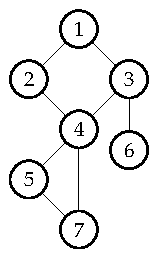
\includegraphics[width=3cm]{graphic1.pdf}
\caption[short]{A problem instance.}
\label{fig:1:b}
\end{subfigure} $\;\;\;$
\begin{subfigure}[t]{.3\linewidth}
\centering
 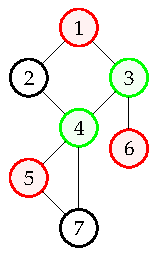
\includegraphics[width=3cm]{graphic2.pdf}
\caption[short]{A feasible solution $\mathcal{D}=\{\{3,4\}, \{1,5,6\}\}$ with $f(\mathcal{D}$)= 0.445.}
\label{fig:1:c}
\end{subfigure} $\;\;\;$
\begin{subfigure}[t]{.3\linewidth}
\centering
 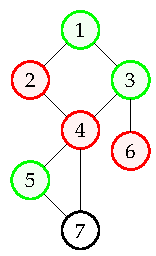
\includegraphics[width=3cm]{graphic3.pdf}
\caption[short]{The optimal solution $\mathcal{D}^*=\{\{1,3,5\},\{2,4,6\}\} $ with $f(\mathcal{D}^{opt}) =0.796$.}
\label{fig:1:d}
\end{subfigure}
\caption{An illustrative example of the MWDDS problem.}
\label{fig:1}
\end{figure}


%\begin{figure}[t]
%\centering
%\subcaptionbox{Table containing the vertex energy-weights. \vspace{0.5 cm} \label{fig:1:a}}[\linewidth]{
%\begin{tabular}{l||ccccccc} \hline
%{\bf vertex label}  & 1 & 2 & 3 & 4 & 5 & 6 & 7 \\ \hline
%{\bf vertex weight} & 0.804 & 0.175 & 0.775& 0.424 & 0.782& 0.021 & 0.257 \\ \hline
%\end{tabular}
%}
%\subcaptionbox{A problem instance.\label{fig:1:b}}[0.3\linewidth]{
% 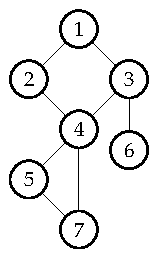
\includegraphics[width=3cm]{graphic1.pdf}
%}\vspace{0.5cm} 
%\subcaptionbox{ A feasible solution $\mathcal{D}=\{\{3,4\}, \{1,5,6\}\}$ with $Lifetime(\mathcal{D}$)= 0.445.\label{fig:1:c}} [0.3\linewidth]{
% 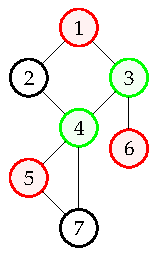
\includegraphics[width=3cm]{graphic2.pdf}
%}\vspace{0.5cm} 
%\subcaptionbox{The optimal solution $\mathcal{D}^{opt}=\{\{1,3,5\},\{2,4,6\}\} $ with $lifetime(\mathcal{D}^{opt}) =0.796$.\label{fig:1:d}}[0.3\linewidth]{
% 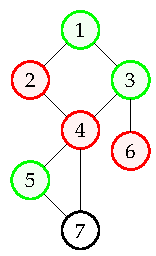
\includegraphics[width=3cm]{graphic3.pdf}
%}
%\caption{An illustrative example of the MWDDS problem.}
%\label{fig:1}
%\end{figure}

\section{An ILP Model for the MWDDS Problem}
\label{sec:ilp-model}

Our ILP model for the MWDDS problem requires the following sets of variables. First, we introduce a binary variable $x_{ij}$ for each node $v_i$ ($i=1,\ldots,n$) and each possible disjoint set $D_j$ ($j=1,\ldots,\delta(G) + 1$). Hereby, $\delta(G) := \min \{deg(v) \mid v \in V\}$.\footnote{Remember that the maximum number of disjoint dominating sets in a graph is $\delta(G) + 1$.} When $x_{ij} = 1$, node $v_i$ is assigned to the $j-$th dominating set. Second, a binary variable $y_j$ ($j=1,\ldots,\delta(G) + 1$) indicates whether or not the $j-$th set is opened. Finally, a real-valued variable $z_j \in [0,M]$ ($M \in \mathbb{R}^+$) stores the weight of the $j-$th dominating set. Hereby, $M := \max \{lifetime(v) \mid v \in V\}$. Based on these variables, the MWDDS can be stated as an ILP in the following way. 

 \begin{align}
    \textbf{max}    \quad  & \sum_{j=1}^{\delta(G)+1} z_j \label{eq2:1} & \\ 
    \textbf{s.~t.}       \quad  & \sum_{j=1}^{\delta(G)+1} x_{ij}  \leq 1 & i = 1,\ldots,n \label{eq2:2} \\
                         \quad  & \sum_{v_k \in N(v_i)} x_{kj} \geq y_j - x_{ij}  & j = 1,\ldots,\delta(G)+1 \label{eq2:3}    \\
                         \quad  & y_j \geq x_{ij}                                 & i = 1,\ldots,n \mbox{ and } j = 1,\ldots,\delta(G)+1 \label{eq2:4} \\
                         \quad  & x_{ij} \cdot lifetime(v_i) + (1 - x_{ij}) \cdot M \geq z_j & i = 1,\ldots,n \mbox{ and } j = 1,\ldots,\delta(G)+1 \label{eq2:5} \\
                         \quad  & y_j \cdot M \geq z_j                       & j = 1, \ldots,\delta(G) + 1 \label{eq2:6} \\
                         \quad  & y_j \geq y_{j+1}                           & j = 1, \ldots,\delta(G) \label{eq2:7} \\
                         \quad  & z_j \geq z_{j+1}                           & j = 1, \ldots,\delta(G) \label{eq2:8}
\end{align}

The objective function sums over the weight values of all dominating sets. Note that, for this objective function to be correct, the weight value of those dominating sets that are not opened must be set to zero by respective constraints. Constraints~(\ref{eq2:2}) require that each node of the graph is assigned to at most one dominating set. This assures the disjointness of the dominating sets. Next, constraints~(\ref{eq2:3}) are the so-called dominating set constraints, that is, they ensure that, if the $j-$th set is opened, then the set of nodes assigned to the $j$-th set form a dominating set of $G$. Further, constraints~(\ref{eq2:4}) make sure that nodes can only be assigned to opened dominating sets. Constraints~(\ref{eq2:5}) are responsible for correctly determining the weights of the openend dominating sets. In other words, the value of variable $z_j$ of the $j-$th dominating set (if open) is set to the minimum of the lifetime-values of all nodes assigned to this set. Next, constraints~(\ref{eq2:6}) ensure that the weight values of dominating sets that are not opened are set to zero. Finally, the last two sets of constraints---that is, constraints~(\ref{eq2:7}) and~(\ref{eq2:8})---are not necessary for the correctness of the ILP. They are tie-breaking constraints that ensure that (1) if $k$ dominating sets are openend, they are assigned to sets $1,\ldots,k$ and (2) the openend dominating sets are ordered according to a non-increasing weight value.

\section{Proposed Greedy heuristic}
\label{sec:greedy}

Greedy algorithms are constructive heuristics for building feasible solutions to combinatorial optimization problems. They start from an empty solution and iteratively add the most favorable component from a set of feasible extensions of the current partial solution until a complete solution is reached. That is, the component to be added at each construction step is chosen deterministically according to some greedy function, which is a measure for the goodness of the solution components. In general, greedy heuristics do not require overly large computation times. The main drawback of a greedy heuristic is that the single constructed solution is most likely not optimal.

 \begin{algorithm}[t]
 \caption{GH-MWDDS: A Greedy heuristic for the MWDDS problem}
  \label{alg:1}
   \begin{normalsize}
   
 \begin{algorithmic}[1]
 \renewcommand{\algorithmicrequire}{\textbf{Input:}}
 \renewcommand{\algorithmicensure}{\textbf{Output:}}
 \REQUIRE a simple, node-weighted, undirected graph $G=(V,E, lifetime)$ 
 \ENSURE  a family of disjoint dominating sets $\mathcal{D} = \{D_{1}, D_{2},\cdots, D_{k} \}$
  \STATE $\mathcal{D}\gets  \emptyset$
  \STATE $k \gets$ 0
  \STATE $V_{\mathrm{rem}} \gets V$
  \STATE $V_{\mathrm{done}} \gets \emptyset$
  \WHILE {not exists $v \in V$ s.t.~$N[v]$ is a subset of $V_{\mathrm{done}}$}
        \STATE $k \gets k + 1$
        \FOR{each node $v \in V$ }
              \STATE $ color(v) \gets $ WHITE
        \ENDFOR   
        \STATE $D_k  \gets \emptyset$ 
        \WHILE  {$D_k$ is not a dominating set of $G$ (that is, $N[D_k] \not= V$)}
               \STATE $v^{*} \gets \text{argmax} \{ score(v) \mid  v \in \{\mathcal{G}(D_k) \cup \mathcal{W}(D_k)\} \cap V_{\mathrm{rem}} \}$                              
               \STATE $D_k \gets D_k \cup \{ v^{*} \}$
               \STATE $V_{\mathrm{rem}} \gets  V_{\mathrm{rem}} \setminus  \{ v^{*} \}$
               \FOR{each node $ u \in N(v^{*})$ }
                 \IF {( $color(u) = $ WHITE )}
                     \STATE $ color(v) \gets $ GRAY
                 \ENDIF
               \ENDFOR 
                \STATE $ color(v^{*}) \gets $ BLACK
                       
        \ENDWHILE
        \STATE \textsf{Reduce}($D_k$, $V_{\mathrm{rem}}$, $V_{\mathrm{done}}$) \COMMENT{optional}
        \STATE $\mathcal{D}\gets  \mathcal{D} \cup  \{ D_k \}$
        \STATE $V_{\mathrm{done}} \gets V_{\mathrm{done}} \cup D_k$
   \ENDWHILE         
        
  \RETURN  $\mathcal{D} = \{D_{1}, D_{2},\cdots, D_{k} \}$.      			
  \end{algorithmic} 
  \end{normalsize}
\end{algorithm}

The pseudo-code of our greedy algorithm, henceforth labelled GH-MWDDS, is presented in Algorithm~\ref{alg:1}. At the start of the algorithm, the following sets are initialized. Solution $\mathcal{D}$ is initialized to the empty set. Furthermore, set $V_{\mathrm{rem}}$, which contains all nodes that may still be added to a dominating set, is initialized to $V$. Finally, set $V_{\mathrm{done}}$, which collects all nodes that already form part of a dominating set in $\mathcal{D}$, is initialized to the empty set. Counter $k$ counts the number of dominating sets that are being constructed. It is initialized to zero. At each main iteration $k \geq 1$, the algorithm generates a dominating set $D_k$ consisting of nodes from set $V_{\mathrm{rem}}$ which, as mentioned above, contains all nodes of $G$ that do not form part of any of the already generated dominating sets $D_i$, $i=1,\ldots, k - 1$; see lines~5 and~21. The algorithm stops once no further dominating set can be generated from the nodes in $V_{\mathrm{rem}}$. This is the case if at least one node $v \in V$ and all its neighbors form part of $V_{\mathrm{done}}$. More formally, the algorithm stops if there is at least one $v \in V$ such that $N[v]$ is a subset of $V_{\mathrm{done}}$ (see line~5).

The construction of a dominating set $D_k$ at round $k$ of the algorithm is done as follows. First, $D_k$ is initialized to the empty set. At each moment, each node of the input graph $G$ belongs to one of the following sets:
\begin{itemize}
  \item  \textit{Black  nodes}: nodes that are part of $D_k$.
  \item  \textit{Gray nodes}: nodes in $\mathcal{G}(D_k) := N(D_k) \setminus D_k$, that is, nodes that are not contained in $D_k$ but that are adjacent to at least one black node.
  \item  \textit{White nodes}: nodes in $\mathcal{W}(D_k) := V \setminus N[D_k]$, that is, nodes that are neither gray nor black.
\end{itemize} 
Remember, in this context, that $N(D_k)$ and $N[D_k]$ denote the open neighborhood and the closed neighborhood of $D_k$, respectively. Given these definitions, $D_k$ is iteratively generated by adding at each construction step exactly one node from $\{\mathcal{G}(D_k) \cup \mathcal{W}(D_k)\} \cap V_{\mathrm{rem}}$, that is, a nodes that is (1) either gray or white, and (2) that is not already added to one of the dominating sets from previous rounds. In order to make this choice, all nodes from $\{\mathcal{G}(D_k) \cup \mathcal{W}(D_k)\} \cap V_{\mathrm{rem}}$ are evaluated by means of greedy function $\textit{score}()$, which is defined as follows:
\begin{align}
	&  \textit{score} (v) :=  lifetime(v) * white\_degree(v)  &  \forall v \in \{\mathcal{G}(D_k) \cup \mathcal{W}(D_k)\} \cap V_{\mathrm{rem}} &   \label{eq3:1} \\
	&  \textit{white\_degree(v)} := \vert N[v] \cap \mathcal{W}(D_k)  \vert &  \label{eq3:2} 
\end{align}
In other words, the greedy function of a node $v$ is obtained by multiplying the lifetime of the node with the number of white nodes from the closed neighborhood of $v$.

%The pseudo-code of our proposed greedy heuristic for MWDDS problem is provided in Algorithm~\ref{alg:1}. It takes as input a problem instance represented as a simple, connected weighted undirected graph $G=(V,E, lifetime)$ with $n$ vertices  and produces as outputs a family of disjoint dominating sets  $\mathcal{D} = \{D_{1}, D_{2},\cdots, D_{k} \}$. It works as follows. At the beginning, the family of disjoint dominating sets is empty and $k = 1$. Let $clist$ represents the set of solution components from which the current dominating set $D_k $ will be generated. Initially, $clist$ contains all vertices of $V$. Then, as in any greedy algorithm, $D_k $ are constructed from scratch by adding, at each step construction, one vertex from $clist$ until $D_k $ is a dominating set. A vertex $v$ is chosen to be included in $D_k$ according to a scoring function $score(v)$ depending both on its energy $lifetime(v)$  and  the number of vertices in its closed neighborhood that are in $\mathcal{W}(D_k)$, calculated as in Equation~(\ref{eq3:1}).


%Finally, the algorithm terminates when no more dominating set can be constructed from the remaining nodes in $clist$ and $\mathcal{D}$ cannot be further extended. Doing so, suppose  that we have already  constructed a  dominating  set $D_k$  at round $k$ and we want to  pursue to construct the next dominating set $D_{k+1}$, to avoid be locked into a partial solution  $D_{k+1}$ that cannot be extended to a complete solution (i.e., a dominating set), we have to check before starting the construction whether there exists a vertex $v$ from $D_1\cup D_1 \cup \cdots  D_k$ that cannot be covered in next round $k+1$, that is $ref\_dom (v) = deg(v) + 1$, where $ref\_dom (v)= \vert \{ u \in N[v]: u \in D_1\cup D_1 \cup \cdots  D_k\}  \vert$ refereed to nodes in the closed neighborhood of $v$ that are part of previous chosen dominating set. Intuitively, if it is the case, then the algorithm terminates in at most $O(m*n)$ time.

To further improve the quality of solutions, the dominating set $D_k$ might be reduced by removing redudant nodes before adding $D_k$ to solution $\mathcal{D}$. This is done in the optional function \textsf{Reduce}$(D_k, V_{\mathrm{rem}}, V_{\mathrm{done}})$; see line~22 of the pseudo-code. Formally, a node $v \in D_k$  is redundant if each node from its closed neighborhood $N[v]$ is dominated by at least two nodes from $D_k$, that is, $N[v] \subset \bigcup_{u \in D_k \setminus \{v\}} N[u]$~\cite{bouamama2016:hybrid}. Redundant nodes are identified and removed in an iterative way. Moreover, sets $V_{\mathrm{rem}}$ and $V_{\mathrm{done}}$ are updated accordingly.

\subsection{Time Complexity of GH-MWDDS}

In this section, we analyze the complexity of our greedy algorithm, without the optional reduction mechanism from line~22. The main while loop (line~5) of the algorithm is iterated $k$ times (rounds), where $k$ refers to the number of disjoint dominating sets returned by the algorithm. Since the maximum number of dominating sets in a domatic partition of a graph $G=(V,E)$ is less or equal to $\delta +1$ \cite{feige2002approximating}, where $\delta$ is the minimum degree of any node of $G$, it holds that $k \leq \delta +1$. As a result, checking the condition in line~5 and executing lines 7-9 is both done in $O(\delta\cdot n)$ time. Further, $n$ is clearly an upper bound for the number of times that the inner while loop (lines 11-21) is iterated. To determine the time complexity of line~12, we proceed as follows. Remember that for any node $v$ the calculation of its $white\_degree(v)$ value requires $deg(v)$ operations. Moreover, for choosing the first node $v^{*}_{1}$ of a dominating set, line 12 requires a time of $deg(v_{1})+ deg(v_{2})+ \cdots + deg(v_{n})$. The well-known Handshaking Lemma states that $\sum\limits_{v \in V} { deg(v)} = 2 m$, where $m = |E|$. For choosing the second node $v^{*}_{2}$, line 12 requires  $m - deg(v^{*}_{1})$ time, etc. Therefore, the total time complexity of line 12 is $O(n\ m)$. In summary, we can conclude that our greedy algorithm has a worst-case time complexity of $O(\delta\ n)+ O(n\ m)= O ( max(\delta\ n, n\ m)) = O(n\ m) $.

\section{Experimental Evaluation}
\label{sec:experiments}

The proposed greedy algorithm (GH-MWDDS) was implemented in ANSI C++ using  GCC~7.4.0 for compiling the software. Its performance was compared with three recent local search approaches available from the related literature~\cite{pino2018:dominating}: Local Search (LS), Fixed Depth (FD), and Variable Depth (VD). In order to conduct a fair comparison to the three local search algorithms (LS, FD and VD) we used the original source code provided by the authors of~\cite{pino2018:dominating}. GH-MWDDS and the three local search algorithms were experimentally evaluated on a laptop equipped with a 64-bit 2.5-GHz Intel{\textregistered} Core\texttrademark ~i5-7200U processor and 8 GB of RAM. We applied GH-MWDDS to a set of 640 problem instances that are described below. Moreover, in order to test the usefulness of our ILP model, we applied the ILP solver ILOG CPLEX 20.01 in single-threaded mode to all problem instances. The time limit for each application of CPLEX was set to 2 CPU hours. Moreover, the experiments with CPLEX were performed on a cluster of machines with two Intel\textsuperscript{\textregistered} Xeon\textsuperscript{\textregistered} Silver 4210 CPUs with 10 cores of 2.20GHz and 92 Gbytes of RAM.

\subsection{Problem Instances}

We used the source code provided in~\cite{pino2018:dominating} for generating 640 diverse problem instances. Each problem instance was generated according to two control parameters: the size of the network $n$ (number of nodes) and its average degree $d$, where $d = 2 m/n$ and $m$ is the number of edges. More specifically, we considered five different network sizes: 50, 100, 150, 200 and 250 nodes. For each network size, we considered between 5 to 8 different average degrees in a way such that networks over a range from sparse to dense networks are generated. In addition, each node (sensor) of the network was given a random real value between 0 and 1 as node weight (lifetime). Then, for each combination of $n$ and $d$, 20 different networks were randomly generated resulting in a total of 640 problem instances for the experimental evaluation. 



\subsection{Results and Discussion}

Table~\ref{tab1:results} reports on the performance comparison of GH-MWDDS (without the optional reduction procedure) and LS, FD, VD, and CPLEX. The first two columns indicate the problem instance type. More specifically, the number of nodes ($n$) is provided in the first column, whereas the average degree ($d$) is shown in the second column. Obviously, the higher $d$, the more dense is the network. Remember that for each combination of $n$ and $d$---that is, for each table row---there are 20 randomly generated problem instances. The values shown in the tables represent the average results obtained for these 20 instances per table row. Table columns~3 and~4 contain the results of CPLEX. While the first one of these columns indicates the average solution quality obtained, the second column provides the average gap (in percent) between the found results and the upper bounds. The results of the other algorithms are provided in two columns for each algorithm. These columns report on the average solution quality (\textit{Value}) and the average computation time (\textit{Time(s)}) in seconds. Moreover, the 11-th column of the table indicates the average size of solutions (${|DP|}$) in terms of the average number of disjoint dominating sets. Since the three algorithms LS, FD and VD start with the same greedy solution as initial solution, and the number of disjoint dominating sets does not change during local search, the column with heading ${|DP|}$ holds for all three algorithms. Finally, in the last column of the table, the average size of the solutions of GH-MWDDS is given. \\

In addition to evaluating GH-MWDDS, we also tested the following two additional versions. Henceforth we refer to the version of GH-MWDDS that removes redundant nodes in line~22 as GH-MWDDS$^{+} $. In addition, the algorithm can be easily adapted in order to solve the maximum disjoint dominating sets (MDDS) problem, instead of the MWDDS. The resulting greedy algorithm, which is called GH-MDDS, is obtained by replacing the $score(\cdot)$ function in line~12 of Algorithm~\ref{alg:1} by the  $white\_degree(\cdot)$  function of Equation~\ref{eq3:2}. The experiential results obtained with GH-MDDS and GH-MWDDS$^{+}$ are provided in Table~\ref{tab2:results}, whose structure is very similar to the one of Table~\ref{tab1:results}.

\end{paracol}

\begin{specialtable}
\widetable
\caption{Numerical results of comparison between LS, FD, VD and GH-MWDDS  \label{tab1:results}}
%MDPI: (1) We helped to add the comma between figures more than 5 digits. Please confirm; (2) Please add the explanation of  bold format.
\begin{footnotesize}
\begin{tabular}{ccccccccccccccccccc} 
\toprule
$n$ & $d$  & \multicolumn{2}{c}{CPLEX} && \multicolumn{2}{c}{LS} && \multicolumn{2}{c}{FD} && \multicolumn{2}{c}{VD}& |DP|& &\multicolumn{3}{c}{GH-MWDDS}\\ 
\noalign{\smallskip}  \cline{3-4}  \cline{6-7} \cline{9-10} \cline{12-13} \cline{16-18}  \noalign{\smallskip}
  &    & Value & Gap(\%) && Value  &  Time(s)  &  &  Value  &  Time(s)  &  & Value  &  Time(s)&  &  & Value  &  Time(s)& |DP| \\ 
\midrule
% Table generated by Excel2LaTeX from sheet 'Global'
 50  & 15   & \bf2.779   & 32.839  &&  0.395  &  0.003  & &  0.477  &  0.019   & &  0.555  &  1.984    & 2.55  & & 2.155  &  0.000 & 5.75 \\
     & 20   & \bf3.922   & 121.088 &&  0.649  &  0.004  & &  0.825  &  0.055   & &  1.014  &  7.651    & 3.55  & & 3.353  &  0.001 & 8.05 \\
     & 25   & \bf5.098   & 158.038 &&  1.011  &  0.006  & &  1.245  &  0.055   & &  1.490  &  4.885    & 4.05  & & 4.595  &  0.001 & 10.05 \\
     & 30   & \bf6.432   & 200.567 &&  1.664  &  0.007  & &  2.460  &  0.124   & &  2.780  &  13.117   & 6.30  & & 5.926  &  0.001 & 12.90 \\
     & 35   & \bf7.929   & 197.434 &&  2.200  &  0.012  & &  2.914  &  0.204   & &  3.166  &  25.048   & 6.85  & & 7.376  &  0.000 & 15.30 \\ \midrule 
 100 & 20   & 2.467   & 405.669 &&  0.283  &  0.023  & &  0.333  &  0.188   & &  0.423  &  30.458   & 2.45  & & {\bf 2.784}  &  0.001 & 7.00 \\
     & 30   & 3.202   & >1000.0 &&  0.431  &  0.017  & &  0.535  &  0.165   & &  0.576  &  31.796   & 2.95  & & {\bf 4.501}  &  0.003 & 10.90 \\
     & 40   & 3.338   & >1000.0 &&  0.859  &  0.021  & &  1.259  &  0.394   & &  1.341  &  183.921  & 4.75  & & {\bf 6.679}  &  0.002 & 14.80 \\
     & 50   & 3.857   & >1000.0 &&  1.361  &  0.038  & &  2.018  &  0.796   & &  2.407  &  225.704  & 6.00  & & {\bf 8.500}  &  0.001 & 18.65 \\
     & 60   & 5.804   & 823.022 &&  2.019  &  0.027  & &  2.884  &  0.830   & &  3.226  &  362.775  & 7.15  & & {\bf 11.131} & 0.001  & 23.40 \\  \midrule
 150 & 30   & 0.055   & >1000.0 &&  0.287  &  0.053  & &  0.326  &  0.316   & &  0.326  &  106.602  & 2.85  & & {\bf 4.098}  &  0.002 & 10.65 \\
     & 40   & 0.028   & >1000.0 &&  0.557  &  0.050  & &  0.670  &  0.595   & &  0.745  &  156.994  & 3.80  & & {\bf 5.816}  &  0.003 & 14.05 \\
     & 50   & 0.011   & >1000.0 &&  0.615  &  0.077  & &  0.927  &  1.139   & &  1.009  &  182.630  & 3.95  & & {\bf 7.479}  &  0.003 & 17.50 \\
     & 60   & 0       & >1000.0 &&  0.848  &  0.046  & &  1.506  &  2.576   & &  1.521  &  646.268  & 4.90  & & {\bf 9.281}  &  0.002 & 21.00 \\
     & 70   & 0       & >1000.0 &&  1.373  &  0.066  & &  2.293  &  4.219   & &  2.464  &  1028.650 & 6.65  & & {\bf 11.388} & 0.004  & 24.45 \\
     & 80   & 0       & >1000.0 &&  1.689  &  0.065  & &  2.729  &  2.599   & &  3.036  &  549.900  & 7.20  & & {\bf 13.508} & 0.005  & 28.90 \\
     & 90   & 0       & >1000.0 &&  2.209  &  0.055  & &  3.817  &  3.793   & &  4.193  &  906.030  & 9.05  & & {\bf 15.485} & 0.006  & 32.95 \\ \midrule
 200 & 40   & 0       & >1000.0 &&  0.256  &  0.049  & &  0.317  &  0.648   & &  0.370  &  81.750   & 2.65  & & {\bf 5.424}  &  0.004 & 13.65 \\
     & 50   & 0       & >1000.0 &&  0.374  &  0.099  & &  0.475  &  1.252   & &  0.483  &  186.900  & 3.45  & & {\bf 6.784}  &  0.005 & 16.60 \\
     & 60   & 0       & >1000.0 &&  0.678  &  0.112  & &  0.897  &  2.083   & &  0.917  &  313.850  & 3.75  & & {\bf 8.656}  &  0.005 & 20.35 \\
     & 70   & 0       & >1000.0 &&  1.004  &  0.170  & &  1.652  &  6.463   & &  1.680  &  3112.950 & 5.95  & & {\bf 10.351} & 0.006  & 23.65 \\
     & 80   & 0       & >1000.0 &&  0.840  &  0.076  & &  1.624  &  5.874   & &  1.795  &  1629.400 & 5.35  & & {\bf 12.447} & 0.008  & 27.15 \\
     & 90   & 0       & >1000.0 &&  1.153  &  0.109  & &  1.924  &  5.260   & &  2.045  &  1364.400 & 5.65  & & {\bf 13.978} & 0.012  & 30.55 \\
     & 100  & 0       & >1000.0 &&  1.503  &  0.091  & &  2.836  &  9.396   & &  3.098  &  3024.830 & 7.65  & & {\bf 15.868} & 0.009  & 34.30 \\ \midrule
 250 & 50   & 0       & >1000.0 &&  0.266  &  0.136  & &  0.314  &  0.867   & &  0.329  &  557.676  & 2.95  & & {\bf 6.681}  &  0.016 & 16.85 \\
     & 60   & 0       & >1000.0 &&  0.526  &  0.221  & &  0.892  &  7.638   & &  0.945  &  1400.788 & 4.55  & & {\bf 8.244}  &  0.012 & 19.70 \\
     & 70   & 0       & >1000.0 &&  0.689  &  0.264  & &  1.050  &  6.906   & &  1.326  &  2380.366 & 5.10  & & {\bf 9.636}  &  0.013 & 22.95 \\
     & 80   & 0       & >1000.0 &&  0.652  &  0.241  & &  1.163  &  9.801   & &  1.445  &  647.763  & 5.40  & & {\bf 11.520} & 0.013  & 26.15 \\
     & 90   & 0       & >1000.0 &&  0.841  &  0.324  & &  1.448  &  18.394  & &  1.591  &  1242.663 & 5.80  & & {\bf 12.938} & 0.013  & 29.55 \\
     & 100  & 0       & >1000.0 &&  1.117  &  0.228  & &  1.981  &  20.789  & &  2.443  &  2210.880 & 6.45  & & {\bf 14.733} & 0.016  & 32.70 \\
     & 120  & 0       & >1000.0 &&  1.259  &  0.146  & &  2.577  &  10.442  & &  2.781  &  2249.350 & 7.20  & & {\bf 18.348} & 0.016  & 39.70 \\
     & 140  & 0       & >1000.0 &&  2.135  &  0.121  & &  4.275  &  16.885  & &  4.713  &  6624.596 & 10.50 & & {\bf 22.478} & 0.020  & 47.25 \\ \midrule
\textbf{Avg} & & 1.404 & && 0.992 &	0.092	& &	 1.583	& 4.399   & &   1.757	 & 984.143	 & 5.231 & & \textbf{9.442}	 &\textbf{ 0.006} & \textbf{21.169} \\
\bottomrule
\end{tabular}
\end{footnotesize}
\end{specialtable}
\begin{paracol}{2}
\switchcolumn


\end{paracol}
\begin{specialtable}
\widetable
\caption{Numerical results of comparison between GH-MDDS, GH-MWDDS and GH-MWDDS$^{+}$ \label{tab2:results}}
\begin{footnotesize}
\begin{tabular}{cccccccccccccc} 
\toprule
$n$ & $d$ && \multicolumn{3}{c}{GH-MDDS} && \multicolumn{3}{c}{GH-MWDDS} && \multicolumn{3}{c}{GH-MWDDS$^{+}$}\\ 
\noalign{\smallskip}  \cline{4-6}  \cline{8-10} \cline{12-14}  \noalign{\smallskip}
  &   & & Value  &  Time(s)  & |DP| & & Value  &  Time(s)  & |DP| & & Value  &  Time(s)  & |DP|  \\ 
\midrule
50 & 15 & &  1.111 & 0.001 & {\bf 6.75}   & &  2.155 & 0.000 & 5.75   & & {\bf 2.191} &   0.002 & 6.150\\
  & 20 & &   1.548 & 0.001 & {\bf 9.05}   & &  3.353 & 0.001 & 8.05   & & {\bf 3.450} &   0.000 & 8.350\\
  & 25 & &   2.630 & 0.001 & {\bf 11.85}  & &  4.595 & 0.001 & 10.05  & & {\bf 4.672} &   0.000 & 10.550\\
  & 30 & &   3.510 & 0.001 & {\bf 14.60}  & &  5.926 & 0.001 & 12.90  & & {\bf 6.042} &   0.000 & 13.350\\
  & 35 & &   4.772 & 0.001 & {\bf 17.25}  & &  7.376 & 0.000 & 15.30  & & {\bf 7.546} &   0.000 & 15.900\\
 \midrule
100 & 20 & & 0.841 & 0.001 & {\bf 8.50}   & &  2.784  & 0.001 & 7.00 & & {\bf 2.842}  &   0.001 & 7.400\\
  & 30 & &   1.714 & 0.004 & {\bf 12.70}  & &  4.501 & 0.003 & 10.90  & &  {\bf 4.580} &   0.001 & 11.150\\
  & 40 & &   2.900 & 0.002 & {\bf 17.15}  & &  6.679 & 0.002 & 14.80  & &  {\bf 6.794} &   0.002 & 15.200\\
  & 50 & &   3.908 & 0.002 & {\bf 21.40}  & &  8.500 & 0.001 & 18.65  & &  {\bf 8.525} &   0.002 & 19.100\\
  & 60 & &   6.111 & 0.004 & {\bf 26.30} & & 11.131  & 0.001 & 23.40  & &  {\bf 11.174} &  0.002 & 23.600\\
    \midrule
150 & 30 & & 1.036 & 0.003 & {\bf 12.00}  & &  4.098 & 0.002 & 10.65  & &  {\bf 4.141} & 0.002 & 10.900\\
  & 40 & &   1.769 & 0.002 & {\bf 16.20}  & &  5.816 & 0.003 & 14.05  & &  {\bf 5.872} & 0.002 & 14.350\\
  & 50 & &   2.553 & 0.003 & {\bf 20.00}  & &  7.479 & 0.003 & 17.50  & &  {\bf 7.570} & 0.002 & 17.850\\
  & 60 & &   3.647 & 0.004 & {\bf 24.10}  & &  9.281 & 0.002 & 21.00  & &  {\bf 9.371} &  0.005 & 21.450\\
  & 70 & &   4.789 & 0.002 & {\bf 28.10}  & & 11.388 & 0.004 & 24.45  & &  {\bf 11.446} &  0.005 & 25.050\\
  & 80 & &   6.468 & 0.005 & {\bf 33.00}  & & 13.508 & 0.005 & 28.90  & &  {\bf 13.611}&  0.003 & 29.150\\
  & 90 & &   7.143 & 0.006 & {\bf 36.55}  & & 15.485 & 0.006 & 32.95  & &  {\bf 15.589}&  0.005 & 33.550\\
    \midrule
 200 & 40 & &   1.350 & 0.006 & {\bf 15.50}  & &  5.424 & 0.004 & 13.65  & &  {\bf 5.486} & 0.005 & 13.950\\
     & 50 & &   1.719 & 0.006 & {\bf 18.95}  & &  6.784 & 0.005 & 16.60  & &  {\bf 6.848} & 0.006 & 17.050\\
     & 60 & &   2.551 & 0.007 & {\bf 23.35}  & &  8.656 & 0.005 & 20.35  & &  {\bf 8.710} & 0.008 & 20.550\\
     & 70 & &   3.566 & 0.008 & {\bf 26.80}  & & 10.351 & 0.006 & 23.65  & &  {\bf 10.395}& 0.008 & 24.100\\
     & 80 & &   4.466 & 0.015 & {\bf 30.70}  & & 12.447 & 0.008 & 27.15  & &  {\bf 12.529}& 0.003 & 27.400\\
     & 90 & &   5.368 & 0.009 & {\bf 34.80}  & & 13.978 & 0.012 & 30.55  & &  {\bf 14.046}& 0.009 & 31.000\\
      & 100 & & 6.425 & 0.011 & {\bf 38.50}  & & 15.868 & 0.009 & 34.30  & &  {\bf 15.993}& 0.009 & 34.650\\
    \midrule
250 & 50 & &   1.643 & 0.013 & {\bf 19.05}  & &  6.681 & 0.016 & 16.85  & &  {\bf 6.783} & 0.008 & 16.950\\
    & 60 & &   2.062 & 0.010 & {\bf 22.70}  & &  8.244 & 0.012 & 19.70  & &  {\bf 8.285} & 0.010 & 19.950\\
    & 70 & &   2.613 & 0.012 & {\bf 26.15}  & &  9.636 & 0.013 & 22.95  & &  {\bf 9.699} & 0.013 & 23.150\\
    & 80 & &   3.348 & 0.013 & {\bf 29.55}  & & 11.520 & 0.013 & 26.15  & &  {\bf 11.571}& 0.013 & 26.500\\
    & 90 & &   4.030 & 0.016 & {\bf 33.50}  & & 12.938 & 0.013 & 29.55  & &  {\bf 12.978}& 0.016 & 29.900\\
   & 100 & &   5.024 & 0.016 & {\bf 37.15}  & & 14.733 & 0.016 & 32.70  & &  {\bf 14.800}& 0.016 & 33.150\\
   & 120 & &   7.134 & 0.017 & {\bf 45.05}  & & 18.348 & 0.016 & 39.70  & &  {\bf 18.418}& 0.018 & 40.250\\
   & 140 & &   9.584 & 0.020 & {\bf 53.60}  & & 22.478 & 0.020 & 47.25  & &  {\bf 22.514}& 0.020 & 47.700\\
   \midrule
\textbf{Avg}  & & & 3.667  & 0.007 & \textbf{24.089}  & & 9.442 & 0.006 & 21.169 & & \textbf{9.515}  &    0.006 & 21.541 \\
\bottomrule
\end{tabular}
\end{footnotesize}
\end{specialtable}
\begin{paracol}{2}
\switchcolumn

From the results displayed in Tables~\ref{tab1:results} and~\ref{tab2:results}, the following observations can me made: 
\begin{itemize}

\item First of all, the ILP model (solved by CPLEX) is only useful in the context of the smallest problem instances. In fact, CPLEX obtains the best results for all networks with 50 nodes. As an additional information we can say that CPLEX was able to solve 8 out of 20 problem instances with 50 nodes and an average degree of 15 to optimality. In contrast, CPLEX already starts to fail for the instances with 100 nodes, for which the results are already inferior to those of GH-MWDDS. In fact, for most of the problem instances (starting from 150 nodes and an average degree of 60) CPLEX is unable to find anything but the trivial solution that contains no dominating set.

\item Concerning GH-MWDDS, we can observe that it dominates the three competitors from the literature for all problem instances in terms of solution quality as well as computational time. It is significantly better than the best of the other three approaches, while requiring a computation time that is approximately five orders of magnitude smaller than the time needed by the other methods. The improvement ratio of our algorithm with respect to VD (the best approach from the literature) is about 5.37.   

\item As expected, most solutions suffer from the existence of redundant nodes. As a result, GH-MWDDS$ ^{+}$ is able to produce solutions whose size (in terms of the number of disjoint dominating sets) is increased with respect to the solutions produced by GH-MWDDS. This is achieved without compromising the quality of the generated solutions. On the contrary, the quality of the obtained solutions is slighly improved, at the cost of a negligible amount of computation time.

\item In addition, from Table~\ref{tab2:results} we can observe that GH-MDDS and GH-MWDDS$^{+}$ achieve an overall average solution quality (see that last row of Table~\ref{tab2:results}) of 3.667  and 9.515, respectively, and an average solution size (in terms of the number of disjoint dominating sets) of 24.089 and 21.541, respectively. It is worthwhile to note that GH-MDDS always produces solutions with the maximum possible size (equal to $\delta(G)+1$). However, the quality of these solutions (as measured by the objective function of the MWDDS problem) is, of course, lower than the quality of the solutions produced by GH-MWDDS. This is because GH-MDDS is primarily focused on finding solutions of large size, without taking into consideration the problem-specific knowledge of the lifetime values of the nodes. Therefore, a solution to the MWDDS problem with the maximum size does not necessarily correspond to the best MWDDS-solution. For example, in the case where $n$ = 250 and $d$ = 140, for which GA-MDDS finds a solutions with an average value 9.584 and an average size 53.6, GH-MWDDS$^{+}$ finds solutions with an average value 22.514 and average size 47.7. 

\item From above observations we can say that the poor performance of the three local search algorithms proposed by Pino et \textit{al.}~\cite{pino2018:dominating} is mainly due to greedy heuristic used for producing the initial solutions for their local search approaches. Since this greedy heuristic was developed for the MDDS problem, and the local search approaches try to improve these solutions by making swaps among nodes of different disjoint dominating sets, they are limited to the size of the solutions found by the initial greedy heuristic, which cannot be changed later. As can be seen by our results, this way of proceeding limits too much the possibility of the local search algorithms to find improvements.
\end{itemize}

In summary we can say that our GH-MWDDS approach is clearly a new state-of-the-art method for the MWDDS problem.



\section{Conclusions}
\label{sec:conclusions}

This paper deals with the network lifetime maximization problem using the approach of computing disjoint dominating sets in a given network in which sensors are characterized by different lifetime values. In other words, we considered a version of the weighted disjoint dominating sets problem. In this context, we have proposed a greedy heuristic that benefits from the use of problem-specific knowledge. To assess the performance of our algorithm, 640 problem instances of different sizes (both sparse and dense graphs) were evaluated and the obtained results were compared with those of three recently published local search algorithms. Computational results show the superiority of our greedy algorithm over recent approaches available from the literature. In addition we stated the considered problem as an integer linear programming model. However, the results of applying CPLEX to solve the model have shown that this approach is only useful for the smallest ones of the considered networks.

In the future we plan to develop well-working metaheuristics on the basis of the developed greedy heuristic in order to further improve the obtained results. Options include ant colony optimization or iterated greedy algorithms, which are both based on the step-by-step construction of solutions. Another line of research will focus on hybrid techniques such as construct, merge, solve \& adapt (CMSA)~\cite{DBLP:journals/cor/BlumDLL16}, which make it possible to take profit from ILP solvers such as CPLEX even in the context of large problem instances.

%These algorithms showed relatively poor performance in comparison to the proposed algorithm  both in term of solution quality and computational time.


%%%%%%%%%%%%%%%%%%%%%%%%%%%%%%%%%%%%%%%%%%%%
\authorcontributions{The authors contributed equally in all aspects of this research. All authors have read and
agreed to the published version of the manuscript}
%%
\funding{This work was supported by project CI-SUSTAIN funded by the Spanish Ministry of Science and Innovation (PID2019-104156GB-I00).}
%%
%%\institutionalreview{In this section, please add the Institutional Review Board Statement and approval number for studies involving humans or animals. Please note that the Editorial Office might ask you for further information. Please add ``The study was conducted according to the guidelines of the Declaration of Helsinki, and approved by the Institutional Review Board (or Ethics Committee) of NAME OF INSTITUTE (protocol code XXX and date of approval).'' OR ``Ethical review and approval were waived for this study, due to REASON (please provide a detailed justification).'' OR ``Not applicable'' for studies not involving humans or animals. You might also choose to exclude this statement if the study did not involve humans or animals.}
%%
%%\informedconsent{Any research article describing a study involving humans should contain this statement. Please add ``Informed consent was obtained from all subjects involved in the study.'' OR ``Patient consent was waived due to REASON (please provide a detailed justification).'' OR ``Not applicable'' for studies not involving humans. You might also choose to exclude this statement if the study did not involve humans.
%%
%%Written informed consent for publication must be obtained from participating patients who can be identified (including by the patients themselves). Please state ``Written informed consent has been obtained from the patient(s) to publish this paper'' if applicable.}
%
%%\dataavailability{In this section, please provide details regarding where data supporting reported results can be found, including links to publicly archived datasets analyzed or generated during the study. Please refer to suggested Data Availability Statements in section ``MDPI Research Data Policies'' at \url{https://www.mdpi.com/ethics}. You might choose to exclude this statement if the study did not report any data.} 
%
\acknowledgments{The authors would like to thank Tayler Pino for providing  the code of the three proposed local search  algorithms; S.~Bouamama is grateful to DGRSDT-MESRS (Algeria), for financial support.}
%
\conflictsofinterest{The authors declare no conflict of interest.} 
%MDPI: Please confirm this part.
%
%%% Optional
%%\sampleavailability{Samples of the compounds ... are available from the authors.}
%
%%%%%%%%%%%%%%%%%%%%%%%%%%%%%%%%%%%%%%%%%%%
%%% Only for journal Encyclopedia
%%\entrylink{The Link to this entry published on the encyclopedia platform.}
%
%%%%%%%%%%%%%%%%%%%%%%%%%%%%%%%%%%%%%%%%%%%
%%% Optional
%\abbreviations{The following abbreviations are used in this manuscript:\\
%
%\noindent 
%\begin{tabular}{@{}ll}
%PIDS & Positive influence dominating set \\
%LD & Linear dichroism
%\end{tabular}}
%
%%%%%%%%%%%%%%%%%%%%%%%%%%%%%%%%%%%%%%%%%%%
%%% Optional
%\appendixtitles{no} % Leave argument "no" if all appendix headings stay EMPTY (then no dot is printed after "Appendix A"). If the appendix sections contain a heading then change the argument to "yes".
%\appendixstart
%\appendix
%\section{}
%\subsection{}
%The appendix is an optional section that can contain details and data supplemental to the main text---for example, explanations of experimental details that would disrupt the flow of the main text but nonetheless remain crucial to understanding and reproducing the research shown; figures of replicates for experiments of which representative data are shown in the main text can be added here if brief, or as Supplementary Data. Mathematical proofs of results not central to the paper can be added as an appendix.
%
%\begin{specialtable}[H] 
%%\tablesize{\scriptsize}
%\caption{This is a table caption. Tables should be placed in the main text near to the first time they are~cited.\label{tab1}}
%%\tablesize{} % You can specify the fontsize here, e.g., \tablesize{\footnotesize}. If commented out \small will be used.
%\begin{tabular}{ccc}
%\toprule
%\textbf{Title 1}	& \textbf{Title 2}	& \textbf{Title 3}\\
%\midrule
%Entry 1		& Data			& Data\\
%Entry 2		& Data			& Data\\
%\bottomrule
%\end{tabular}
%\end{specialtable}
%
%\section{}
%All appendix sections must be cited in the main text. In the appendices, Figures, Tables, etc. should be labeled, starting with ``A''---e.g., Figure A1, Figure A2, etc. 

%%%%%%%%%%%%%%%%%%%%%%%%%%%%%%%%%%%%%%%%%%
\end{paracol}

\reftitle{References}

% Please provide either the correct journal abbreviation (e.g. according to the “List of Title Word Abbreviations” http://www.issn.org/services/online-services/access-to-the-ltwa/) or the full name of the journal.
% Citations and References in Supplementary files are permitted provided that they also appear in the reference list here. 

%=====================================
% References, variant A: external bibliography
%=====================================
\externalbibliography{yes}
\bibliography{ref}
%%%%%%%%%%%%%%%%%%%%%%%%%%%%%%%%%%%%%%%%%%
\end{document}










\begin{figure}[H]
\centering
\captionsetup[subfigure]{justification=centering}

\subcaptionbox{Table containing the vertex energy-weights. \vspace{0.5 cm} \label{fig:1:a}}{
\begin{tabular}{l||ccccccc} \hline
{\bf node label}  & 1 & 2 & 3 & 4 & 5 & 6 & 7 \\ \hline
{\bf node weight} & 0.804 & 0.175 & 0.775& 0.424 & 0.782& 0.021 & 0.257 \\ \hline
\end{tabular}
}

\subcaptionbox{A problem instance \vspace{0.5 cm} \label{fig:1:b}}[0.3\linewidth]{
   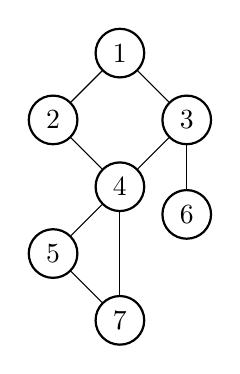
\begin{tikzpicture}[node distance=12 mm]
                \tikzstyle{every node}= [fill=white,draw=black, minimum size=6mm,circle, thick ]
                \node (1)  {1};
                \node (2) [below left of=1] {2};  %\color{red}
		        \node (3) [below right of=1] {3};
		         \node (4) [below right of=2] {4};
		        \node (6) [below of=3] {6};
		        \node (5) [below left of=4] {5};
		        \node (7) [below  right of=5] {7};
		        
                 \path [-,black,thin](1) edge (2)
		                                 edge (3)
		                              (3) edge (4)
		                                  edge (6)
		                              (2) edge (4)   
		                              (4) edge (5)
		                                  edge (7)
		                              (5) edge (7);      	          
\end{tikzpicture}  
}
\hspace*{\fill}
\subcaptionbox{ A feasible solution $\mathcal{D}=\{\{3,4\}, \{1,5,6\}\}$ with $Lifetime(\mathcal{D}$)= 0.445.  \label{fig:1:c}} [0.48\linewidth]{
 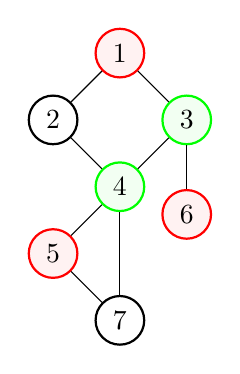
\begin{tikzpicture}[node distance=12 mm, greennode/.style={circle, draw=green, fill=green!5, thick, minimum size=6mm},
 rednode/.style={circle, draw=red, fill=red!5, thick, minimum size=6mm},  blacknode/.style={circle, draw=black, fill= white, thick, minimum size=6mm}, ]   
              
                \node[rednode] (1) {1}; 
                \node [blacknode] (2) [below left of=1] {2};  
		        \node [greennode]  (3)  [below right of=1] {3}; 
		         \node [greennode] (4) [below right of=2] {4};
		        \node [rednode](6) [below of=3] {6};
		        \node [rednode]  (5) [below left of=4] {5}; 
		        \node [blacknode] (7) [below  right of=5] {7};
		        
                 \path [-,black,thin](1) edge (2)
		                                 edge (3)
		                              (3) edge (4)
		                                  edge (6)
		                              (2) edge (4)   
		                              (4) edge (5)
		                                  edge (7)
		                              (5) edge (7);      	          
\end{tikzpicture}    
}


\subcaptionbox{The optimal solution $\mathcal{D}^{opt}=\{\{1,3,5\},\{2,4,6\}\} $ with $lifetime(\mathcal{D}^{opt}) =0.796$.    \label{fig:1:d}}[0.6\linewidth]{
  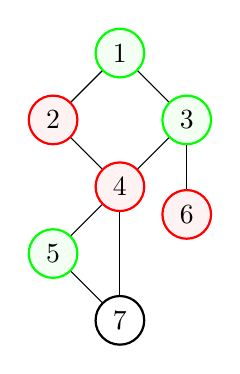
\begin{tikzpicture}[node distance=12 mm, greennode/.style={circle, draw=green, fill=green!5, thick, minimum size=6mm},
 rednode/.style={circle, draw=red, fill=red!5, thick, minimum size=6mm},  blacknode/.style={circle, draw=black, fill= white, thick, minimum size=6mm}, ]   
              
                \node[greennode] (1) {1}; 
                \node [rednode] (2) [below left of=1] {2};  
		        \node [greennode]  (3)  [below right of=1] {3}; 
		         \node [rednode] (4) [below right of=2] {4};
		        \node [rednode](6) [below of=3] {6};
		        \node [greennode]  (5) [below left of=4] {5}; 
		        \node [blacknode] (7) [below  right of=5] {7};
		        
                 \path [-,black,thin](1) edge (2)
		                                 edge (3)
		                              (3) edge (4)
		                                  edge (6)
		                              (2) edge (4)   
		                              (4) edge (5)
		                                  edge (7)
		                              (5) edge (7);      	          
\end{tikzpicture}    
}
\caption{An illustrative example of the MWDDS problem.}
\label{fig:1}
\end{figure}


 \begin{algorithm}[t]
 \caption{GH-MWDDS: A Greedy heuristic for the MWDDS problem}
  \label{alg:1}
   \begin{normalsize}
   
 \begin{algorithmic}[1]
 \renewcommand{\algorithmicrequire}{\textbf{Input:}}
 \renewcommand{\algorithmicensure}{\textbf{Output:}}
 \REQUIRE a simple, node-weighted, undirected graph $G=(V,E, lifetime)$ 
 \ENSURE  a family of disjoint dominating sets $\mathcal{D} = \{D_{1}, D_{2},\cdots, D_{k} \}$
  \STATE $\mathcal{D}\gets  \emptyset$
  \STATE $k \gets$  1
  \STATE $last\_round  \gets$ false
  \WHILE {(not $ last\_round $ )}
        \FOR{each  vertex $ v \in V$ }
              \STATE $ color(v) \gets $ WHITE
        \ENDFOR   
        \STATE $D_k  \gets \emptyset$ 
        \WHILE  {($D_k$ is not a dominating set : $ N(D_k) \neq \emptyset$)}
               \STATE $v^{*} \gets \text{argmax} \{ score(v) \mid  v \in clist \}$                              
               \STATE $D_k \gets D_k \cup \{ v^{*} \}$
               \STATE $ clist \gets  clist  \setminus  \{ v^{*} \}$
               \FOR{each  vertex $ u \in N(v^{*})$ }
                 \IF {( $color(u) = $ WHITE )}
                     \STATE $ color(v) \gets $ GRAY
                 \ENDIF
               \ENDFOR 
                \STATE $ color(v^{*}) \gets $ BLACK
                       
        \ENDWHILE
        \STATE $\mathcal{D}\gets  \mathcal{D} \cup  \{ D_k \}$
        \IF { ( $\exists v \in D_1\cup D_1 \cup \cdots  D_k$ such that $ref\_dom (v) = deg(v) + 1$) } 
          \STATE $ last\_round \gets$  true
          \ELSE 
             \STATE $ k \gets k + 1$
        \ENDIF 
   \ENDWHILE         
        
  \RETURN  $\mathcal{D} = \{D_{1}, D_{2},\cdots, D_{k} \}$.      			
  \end{algorithmic} 
  \end{normalsize}
\end{algorithm}

